\documentclass{article}
\usepackage[utf8]{inputenc}
\usepackage[T1]{fontenc}
\usepackage{graphicx}
\usepackage{hyperref}
\usepackage{geometry}
\geometry{margin=1in}

\title{COI I 130  COI}
\date{Encyclopaedia Britannica (1771)}

\begin{document}
\maketitle

\section*{Historical source}
\textbf{Entry ID:} \texttt{entry-coi-i-130-coi-1250} \\
\textbf{Volume ID:} 149979156 \\
\textbf{Character Count:} 6309

\subsection*{Extracted Text}
Coin,
According to the decouple pre-
portion, mentioned by Livy and Julius Pollox, worth

According to the proportion mentioned by Hectus, and which afterwards obtained, whereby the aurer exchanged for \_5\_ denarii its value

Coin, in architecture, a kind of are cut diagonal, wife, after the manner of a flight of a fluid-cafe, fering in bottom to support columns in a level, and at top to correct the inclination of an entalature fuip- putting a room.

Coin is allo uled for a field angle compofol of two surfaces inclined towards each other, whether that angle be exterior, as the coin of a wall, a tree, fcc or interior, as the coin of a chamber or chimary. See Qouo.

COINAGE, or Coining, the art of making ma-ery, as performed either by the hammer or mill.

Remedy the fabric of coins was different from what it is not present. They cut a large piece of metal into federal little figures, the corners of which were cut with shellsers. After having flapped thefele pieces, fo an are reader than perfectly comfortable, point of weight, to the flandard piece, they took each piece in hand again, to make it seemed young people gentle hummering. This was called \_Adenez\_, and was fit for immediate coming. Then engravers pre-panda, if they fill do, a couple of fleer fits in form of dyes, cut and terminated by flat surface, rounded off at the edges. They engraved or flamped on it the hollow of a head, a cois, a tutendeos, or any other figure, according to to the uniform, the time, with a short legend. As one of thefe dyas was to remain dormant, and the other movable, the former cold in a future prints, this it might be intended into the square hole of the blocks, which, bring fixed very fall, kept the eyes in theory as any vice could have done. The planet of metal has horizontally had upon this inferior mals, to receive the thamp of it on one file, and that of the new dye, wherewith it was covered, on the other. This invisible dye, taking its rough engraved furthest-wing upon the plancher; had at its opposite extremity in flat figures, and larger furties upon which they gave fewer lines show, with a hammer of an enormous fire, till the double thamp was sufficiently, in relleys impressed on each side of the planehet. This being finished, was immediately succeeded by another, and only thus because a functione coin, which had the degree of lineards of the weight and mark, determined by the judgment of the infectors, to make it good current money. The strong tem-pening was wasd is still given to the two dyes, rendering them capable of bearing those expected blows. Coining has been considered, improved and rendered repetitions, by several ingonous machines, and by a wile application of the forell physical expriments to the methods of fixing, drying, and flamping the different results.

The three finest influences the white-man ufes, are the laminating engines: the machine for making the imperfections on the edges of coins, and that null.

After they have taken the laminae, or plates of me-

tal, out of the mould into which they are cafts, they do not best them on the avril, as was formerly done, but they make them pals and repuls between the fe- veral rollers of the laminating engine, which being gradually brought before and defer to the other pro- fently give the lamina its uniform and exact thickensful. Indeed of dividing the lamina can final figures, they at once even clean out of it as many plantaches as it can contain, by means of a sharp fleet trepan, of a roun- dill figure, hollow within, and of a properizationable diameter, to shape and cut of the pieces at one unit the fames times. After theft glances have been prepared and weighed with witharded pieces, flid or forged to get of the greythours part of the metal, and then boiled and made clear, they arrive, at half, at the mas- chine (fig. r.), which marks them when the edge's and flaming the mail (fig. z). which, squeezing each of them flying between the two dyes, brought near each other with one blow, forces the two furfaces or fields of the piece to fill exactly all the vacations of the two figures engraved hollow. The engine which favors to laminate lead, gives a sufficient notion of that which ferns to flatter gold and fiber: laminae between rollers of a kifefer.

The principal pieces of the machine (fig. x.), to damp coins on the edges, are two fiecl laminae, about a fine thick. One half of the legends, of the ring, is engraved on the thickness of one of the laminain, and the other half on the thickelsof the other; and their two laminar and freightly, although the phanchet marked with them he circular.

When they flump a planches, they fril put it be- borne the flavor in flakes as manas, as that the foils- ing cell of them laid flat upon a scrapeplate, which is faltered upon a every thick wooden table, and the phanche being likewise, laid as the tape of the phanchet may take the time liman or each ride, and in their thick part.

One of the fine lamina isimmorable, and faltered the fewralferesys the other lides by menas of a dented wheel, which takes into the teeth that are on the furties of the laminain. This fitting lamin makes the phanchet runs in flash a mansmy that it remains damaged on the edge, when it has made one turn. Only crown and half-croony pieces can lay the im- prefinion of letters on the thickets of their edges.

The cooling engine or mill is for handy (fig. z.), tuna a fragile man may many twenty thousand plants in one day; golg filters and copper planchets, are all of them cooked with a milk, which the coating liquures (fig. z.), commonly called dyes, are flattened; that of the face under, in a figure box garnified with male and female flowers, to fix and keep it flexily and the other above, in a little box garnished with the fame foresew, to fatten the coming liquare. The plan- chet is laid flat on the liquure of the digty, which is manam; and theý immediately pull the bar of the mill by its cords, which can confer the frewef fet within it to turn. This enters into the female fever, which is in the body of the mill and turns with in each through, that by pushing the upper liquare upon that of the effigor, the plainly violently prefilled between both figures, receives the important of both at one pull, and in the twinkling of an eye.

\subsection*{Matched Wikipedia Article}
\textbf{Title:} COI \\
\textbf{Page ID:} 629195 \\
\textbf{Revision ID:} 1160908771 \\
\textbf{URL:} \url{https://en.wikipedia.org/wiki/COI}


\section*{Source record}
\begin{itemize}
\item \textbf{Dataset:} \texttt{NationalLibraryOfScotland/encyclopaedia\_britannica\_illustrated}
\item \textbf{Dataset Revision:} \texttt{309f765b1ecc83e0a7f7762e44b4a927a7555443}
\item \textbf{Page ID:} \texttt{britannica:309f765b1ecc83e0a7f7762e44b4a927a7555443:train:1250} \\
  \textbf{Filename:} \texttt{page-1250-2e0c75f85418.jpg} \\
  \textbf{Row Index:} 1250 \\
  \textbf{SHA256:} \texttt{2e0c75f854185185...}
\end{itemize}

\begin{figure}[h]
\centering
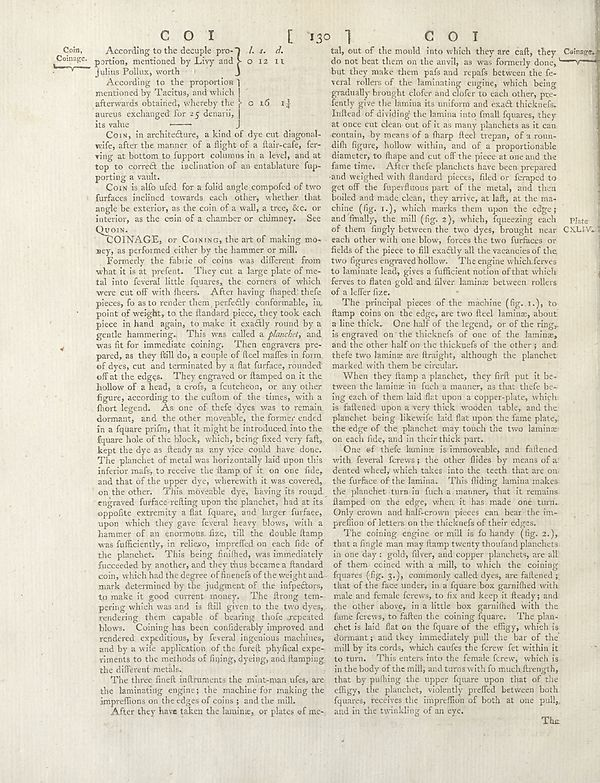
\includegraphics[width=0.85\textwidth]{../scans/page-1250-2e0c75f85418.jpg}
\caption*{Source scan: \texttt{page-1250-2e0c75f85418.jpg}}
\end{figure}

\end{document}
